	\begin{columns}[t,totalwidth=\twocolwid] % Split up the two columns wide column
		
		\begin{column}{0.47\twocolwid}%\vspace{-.6in} % The first column within column 2 (column 2.1)
			\begin{figure}
				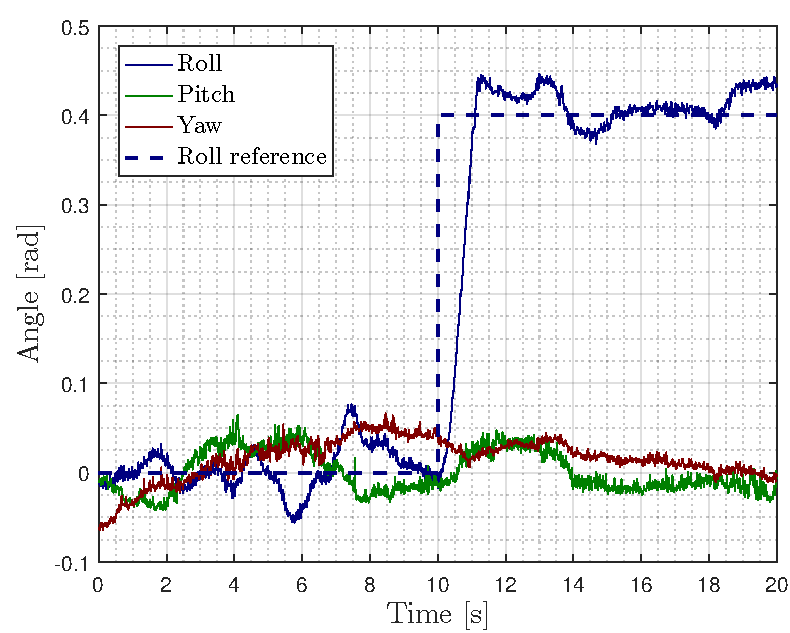
\includegraphics[width=0.8\linewidth]{figures/AttitudeControl}
				\caption{Figure caption}
			\end{figure}
		\end{column} % End of column 2.1
		
		\begin{column}{0.47\twocolwid}%\vspace{-.6in} % The second column within column 2 (column 2.2)
			\begin{figure}
				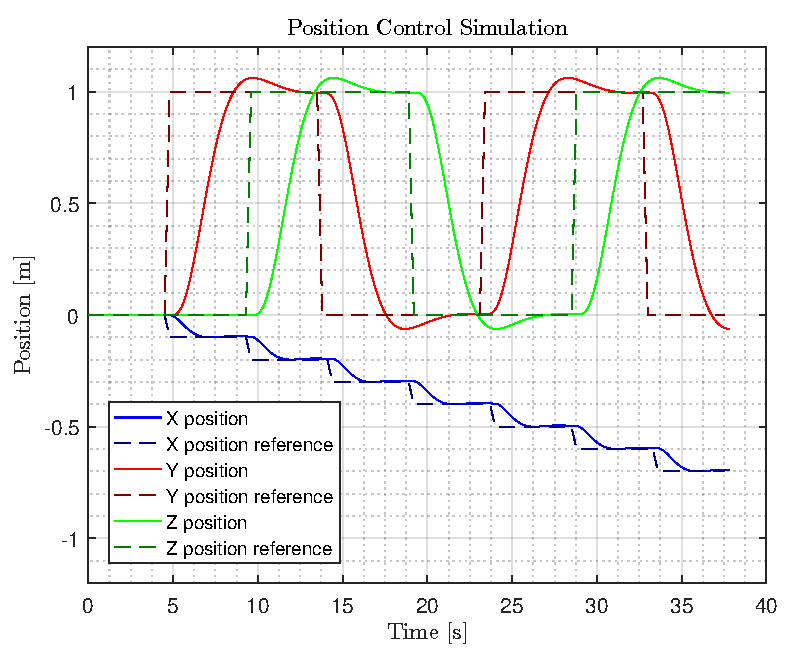
\includegraphics[width=0.8\linewidth]{figures/PositionControl}
				\caption{Figure caption}
			\end{figure}	
		\end{column} % End of column 2.2
		
	\end{columns} % End of the split of column 2 - any content after this will now take up 2 columns width